\subsection{Models}
To implement an API for the WordCount database we needed models for the objects we would be sending and recieving from the other layers. We also needed models corresponding to the database tables to access it through EF Core. The models we have created for communication with other layers and for data access will be described in the following sections.

\subsubsection*{Communication models}
For communication between our layer and the other layers, we have made 3 input, and 1 response model. These models correspond to the JSON objects we expect to send or recieve from other layers when they attempt to insert or retrive data from the database. 
\\
\textbf{Input models}\\
% ArticleJsonModel
% TermJsonModel

The first input model is the ArticleJsonModel which can be seen in figure \ref{ArticlJsonModel}. Article

\begin{figure}[H]
    \centering
    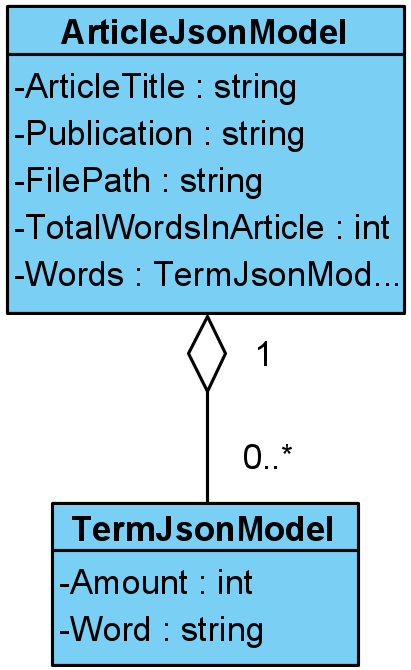
\includegraphics[scale=0.25]{Images/jsonArticleModel.PNG}
    \caption{ArticlJsonModel}
    \label{ArticlJsonModel}
\end{figure}

% JsonSchemaInputModel

\begin{figure}[H]
    \centering
    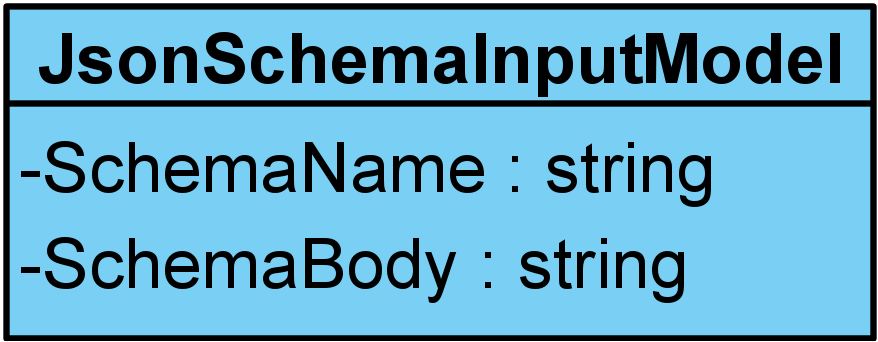
\includegraphics[scale=0.25]{Images/JsonSchemaInputModel.png}
    \caption{JsonSchemaModel}
    \label{JsonSchemaModel}
\end{figure}

\textbf{Response Models}\\
% FileIdResponse

\begin{figure}[H]
    \centering
    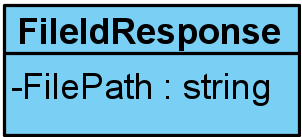
\includegraphics[scale=0.25]{Images/FileIdResponse.png}
    \caption{FileIdResponse}
    \label{FileIdResponse}
\end{figure}

\subsubsection*{Data access models}
We also had to create models for accessing the database through EF Core.

% Article
% publisher
% Term

\begin{figure}[H]
    \centering
    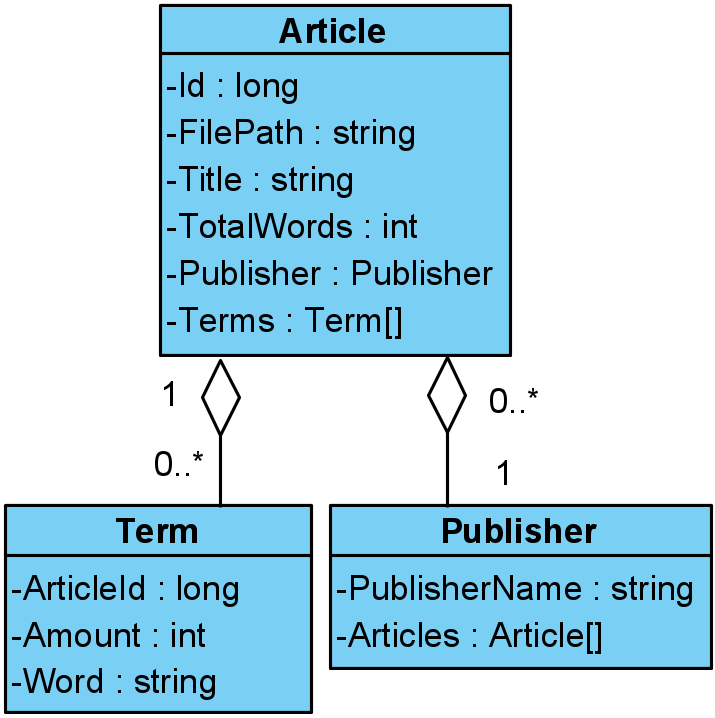
\includegraphics[scale=0.25]{Images/ArticleModel.PNG}
    \caption{Article}
    \label{Article}
\end{figure}

% JsonSchemaModel

\begin{figure}[H]
    \centering
    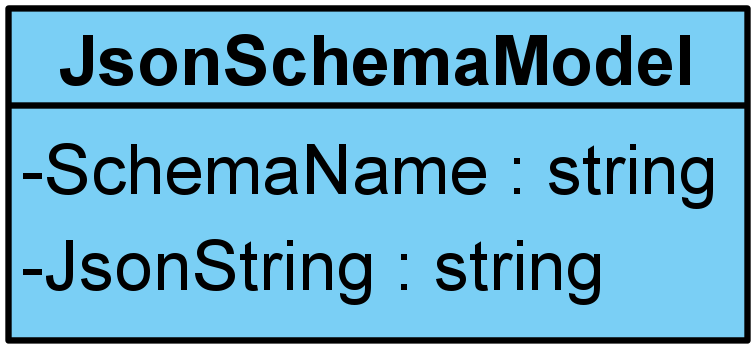
\includegraphics[scale=0.25]{Images/JsonSchemaModel.png}
    \caption{JsonSchemaModel}
    \label{JsonSchemaModel}
\end{figure}

% WordRatio

\begin{figure}[H]
    \centering
    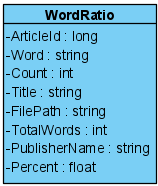
\includegraphics[scale=0.25]{Images/WordRatioModel.png}
    \caption{WordRatioModel}
    \label{WordRatioModel}
\end{figure}